% %%%%%%%%%%%%%%%%%%%%%%%%%%%%%%%%%%%%%%%%%%%%%%%%%%%%%%%%%%%%%%%%%%%%%%%%%%%%%
\chapter{Non-autoregressive NMT with Connectionist Temporal Classification}
\label{chap:nar-nmt-ctc}
% %%%%%%%%%%%%%%%%%%%%%%%%%%%%%%%%%%%%%%%%%%%%%%%%%%%%%%%%%%%%%%%%%%%%%%%%%%%%%



% -----------------------------------------------------------------------------
\section{Connectionist Temporal Classification}
\label{sec:ctc}
% -----------------------------------------------------------------------------

\Gls{ctc} \citep{graves2006connectionist} is a method for training neural
networks on sequential data. Originally applied to the phonetic labelling task,
but later successfully adapted in related areas, including \gls{asr} or
handwriting recognition \citep{liwicki2007novel, eyben2009speech,
  graves2014towards}.

The main strength of \gls{ctc} becomes evident in tasks where the input and
output labels are weakly or not at all aligned, for example in situations where
the observed input sequence is considerably longer than the target output
sequence -- hence the application to \gls{asr}, where the number of extracted
features per second is higher than the number of phonemes uttered per second.
\JH{Confirm this.}

Training neural networks with \gls{ctc} is independent on the actual neural
network architecture. The \gls{ctc} loss function can be applied on any network
with sequential outputs. Thus, this method is applicable to both \glspl{rnn}
and the Transformer model.

Models trained with the \gls{ctc} assume that the alignment between the input
(e.g. a group of frames in an audio signal) and the output (e.g. a phoneme)
states is unknown. A variable number of frames in a row can encode a single
phoneme. Similarly, in translation, multiple words in the source language may
correspond to a single or more words in the target language.

The idea behind \gls{ctc} is to allow some states to produce no output. This is
realized by introducing a special blank token in the target vocabulary.
Optionally, identical outputs produced by multiple consecutive states may be
merged and considered a single output. Because of these properties, there are
groups of equivalent output sequences, which all represent the same target, as
illustrated in Figure~\ref{fig:ctc-equivalent-sequences}.

\begin{figure}
  \centering
  \begin{minipage}{\textwidth}
    \begin{equation*}
        \text{a cat sat on a mat} =
        \begin{cases}
          & \text{a <blank> cat sat on a <blank> mat} \\
          & \text{a a cat cat sat on a mat} \\
          & \text{a <blank> cat cat sat on a mat} \\
        \end{cases}
    \end{equation*}
  \end{minipage}
  \caption{A group of output sequences of equal length which all represent the
    same target in CTC.} %
  \label{fig:ctc-equivalent-sequences}
\end{figure}

In the standard sequence-to-sequence architectures, the value of the loss
function is defined as the sum of the cross entropies of each output state with
respect to the target sequence (see Equation \ref{eq:loss}). In \gls{ctc}, the
loss is defined as the sum of cross-entropy losses of all of the output
sequences equivalent to the given target sequence:
%
\begin{equation}
  J_{\theta}^{\text{CTC}} = - \sum_{(x, y) \in D} \sum_{y' \sim y}  \log p(y' | x, \theta)
  \label{eq:ctc-loss}
\end{equation}
%
where $\sim$ denotes the equivalence relation.  \JH{$J_{\theta}$ should perhaps
  be $J(\theta)$. Also, consider the $\sim$ sign.}

The inner summation in Equation \ref{eq:ctc-loss} is computed over all possible
sequences equivalent to the label sequence. For technical purposes, the label
sequences are limited to a fixed length, which greatly reduces the number of
acceptable hypotheses. However, the number of equivalent hypotheses of a given
length grows exponentially with the sequence length, because in \gls{ctc}, the
fixed length is always set to be longer than the label sequence.

The summation summation over the large set of equivalent sequences can be
implemented using dynamic programming. When both the length of the output and
the length of the target sequences are known, there is a constant number of the
blank tokens to be generated. The process of computing the loss of the whole
output sequence is divided into computing the partial losses with respect to
the possible label prefixes. The \gls{ctc} loss computation is illustrated in
Figure \ref{fig:ctc-dynamic-programming}. Each node in the graph represents

\begin{figure}
  \centering

  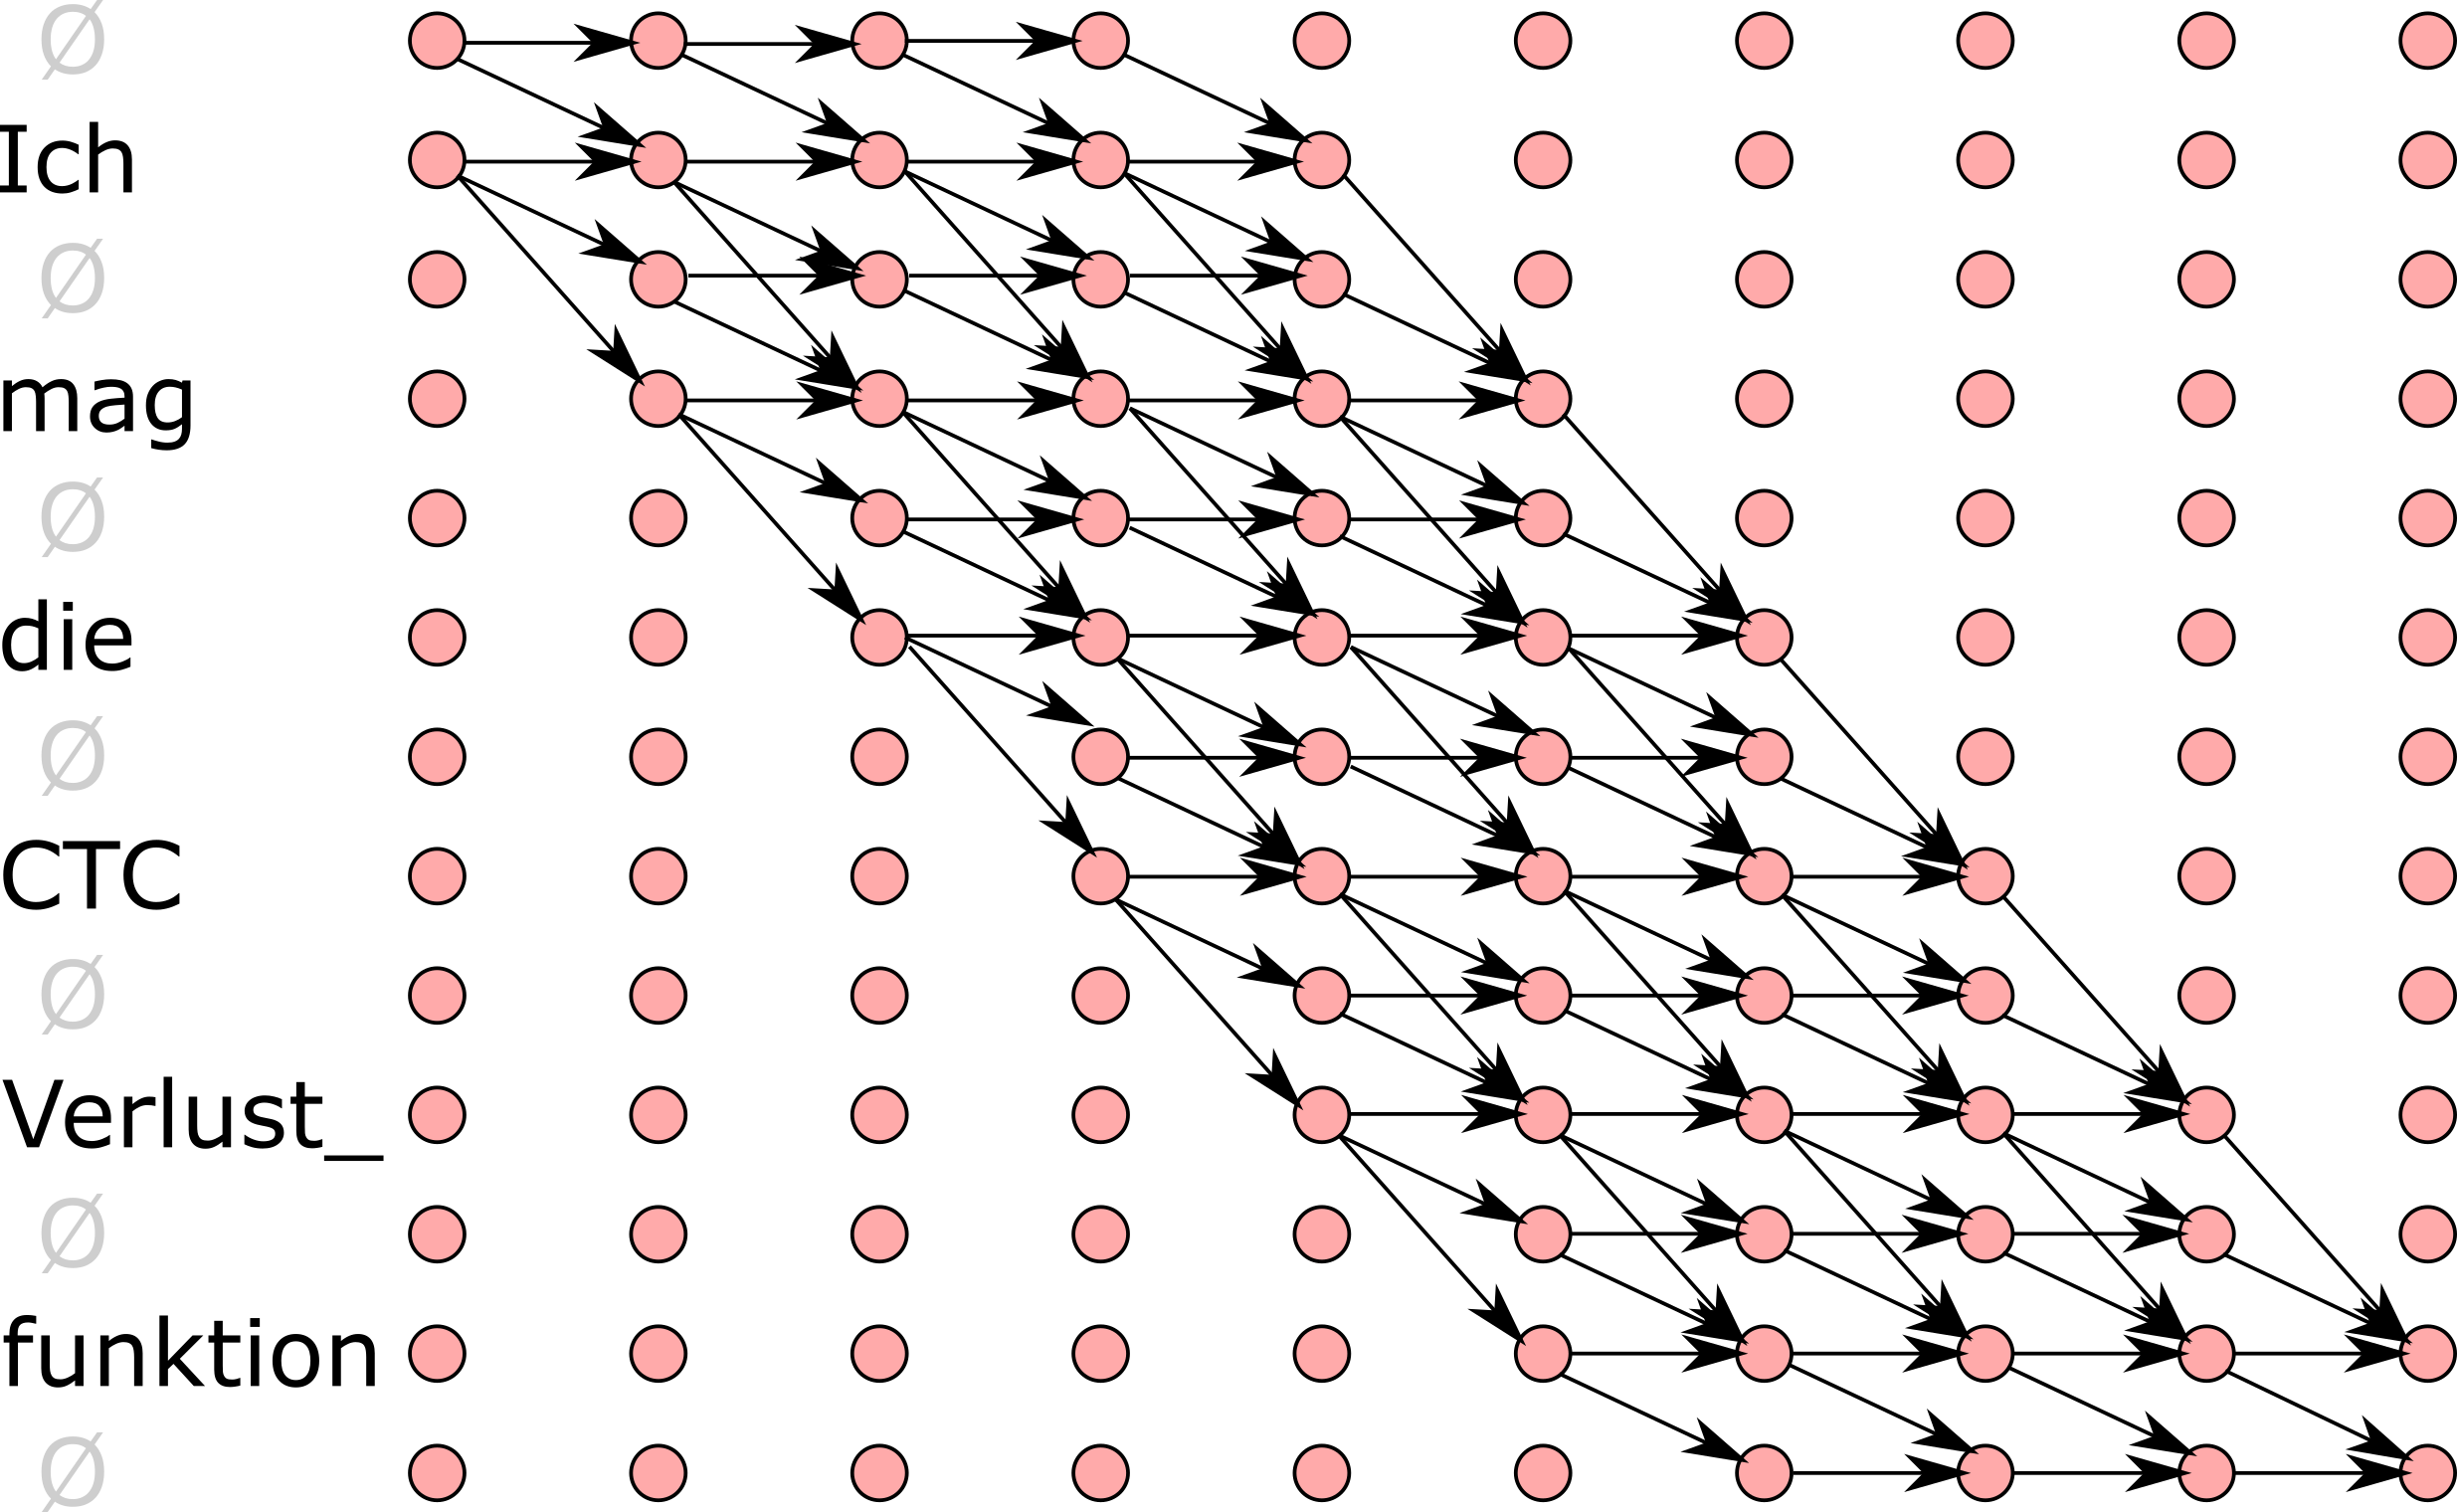
\includegraphics[width=13cm]{img/ctc_schema.png}

  \caption{An illustration of the algorihm for the CTC loss computation. Each
    node denotes producing either a token from the label sequence, or the blank
    token. Each path from one of the two top-left nodes to one of the two
    bottom-right nodes corresponds to one of the equivalent sequences.  }
  \label{fig:ctc-dynamic-programming}
\end{figure}


The training of the network with \gls{ctc} is done
by minimizing the \gls{ctc} loss function, which is defined as follows.



%%% Local Variables:
%%% mode: latex
%%% TeX-master: "thesis"
%%% End:
